\begin{figure}[h]

\tikzset{every picture/.style={line width=0.75pt}} %set default line width to 0.75pt        

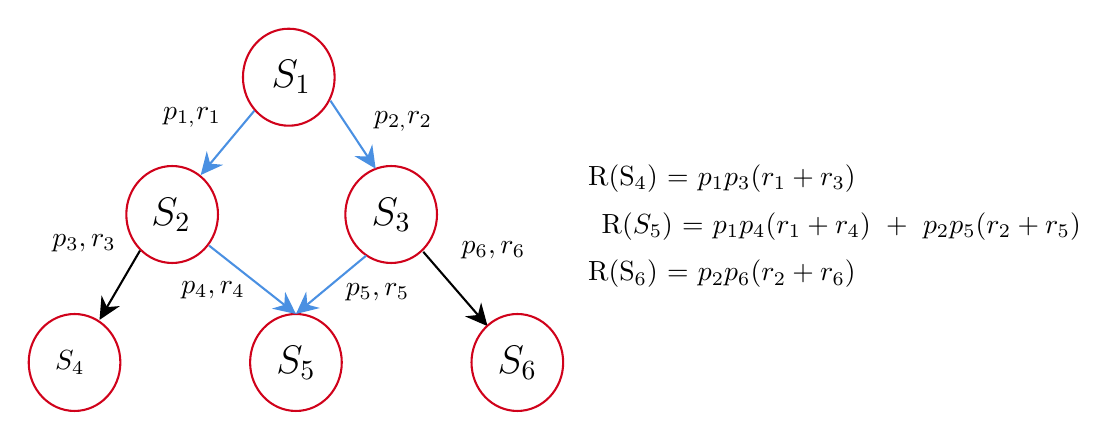
\begin{tikzpicture}[x=0.75pt,y=0.75pt,yscale=-1,xscale=1]
%uncomment if require: \path (0,701.1666717529297); %set diagram left start at 0, and has height of 701.1666717529297

%Straight Lines [id:da8481931635460052] 
\draw    (237.61,125.34) -- (266.62,158.87) ;
\draw [shift={(268.58,161.14)}, rotate = 229.14] [fill={rgb, 255:red, 0; green, 0; blue, 0 }  ][line width=0.08]  [draw opacity=0] (10.72,-5.15) -- (0,0) -- (10.72,5.15) -- (7.12,0) -- cycle    ;

%Shape: Ellipse [id:dp5338816690194331] 
\draw  [color={rgb, 255:red, 208; green, 2; blue, 27 }  ,draw opacity=1 ] (150.73,41.2) .. controls (150.73,28.29) and (160.61,17.83) .. (172.81,17.83) .. controls (185,17.83) and (194.89,28.29) .. (194.89,41.2) .. controls (194.89,54.1) and (185,64.56) .. (172.81,64.56) .. controls (160.61,64.56) and (150.73,54.1) .. (150.73,41.2) -- cycle ;
%Shape: Ellipse [id:dp08323298529021306] 
\draw  [color={rgb, 255:red, 208; green, 2; blue, 27 }  ,draw opacity=1 ] (94.53,107.34) .. controls (94.53,94.44) and (104.41,83.98) .. (116.61,83.98) .. controls (128.8,83.98) and (138.69,94.44) .. (138.69,107.34) .. controls (138.69,120.24) and (128.8,130.7) .. (116.61,130.7) .. controls (104.41,130.7) and (94.53,120.24) .. (94.53,107.34) -- cycle ;
%Shape: Ellipse [id:dp5782501569753735] 
\draw  [color={rgb, 255:red, 208; green, 2; blue, 27 }  ,draw opacity=1 ] (200.05,107.34) .. controls (200.05,94.44) and (209.94,83.98) .. (222.13,83.98) .. controls (234.32,83.98) and (244.21,94.44) .. (244.21,107.34) .. controls (244.21,120.24) and (234.32,130.7) .. (222.13,130.7) .. controls (209.94,130.7) and (200.05,120.24) .. (200.05,107.34) -- cycle ;
%Shape: Ellipse [id:dp9542564413163499] 
\draw  [color={rgb, 255:red, 208; green, 2; blue, 27 }  ,draw opacity=1 ] (47.5,178.64) .. controls (47.5,165.74) and (57.39,155.28) .. (69.58,155.28) .. controls (81.77,155.28) and (91.66,165.74) .. (91.66,178.64) .. controls (91.66,191.54) and (81.77,202) .. (69.58,202) .. controls (57.39,202) and (47.5,191.54) .. (47.5,178.64) -- cycle ;
%Shape: Ellipse [id:dp5730745954231323] 
\draw  [color={rgb, 255:red, 208; green, 2; blue, 27 }  ,draw opacity=1 ] (154.17,178.64) .. controls (154.17,165.74) and (164.06,155.28) .. (176.25,155.28) .. controls (188.44,155.28) and (198.33,165.74) .. (198.33,178.64) .. controls (198.33,191.54) and (188.44,202) .. (176.25,202) .. controls (164.06,202) and (154.17,191.54) .. (154.17,178.64) -- cycle ;
%Shape: Ellipse [id:dp08303160892055261] 
\draw  [color={rgb, 255:red, 208; green, 2; blue, 27 }  ,draw opacity=1 ] (260.84,178.64) .. controls (260.84,165.74) and (270.73,155.28) .. (282.92,155.28) .. controls (295.11,155.28) and (305,165.74) .. (305,178.64) .. controls (305,191.54) and (295.11,202) .. (282.92,202) .. controls (270.73,202) and (260.84,191.54) .. (260.84,178.64) -- cycle ;
%Straight Lines [id:da4561249701318062] 
\draw    (101.12,124.73) -- (83.14,155.52) ;
\draw [shift={(81.62,158.11)}, rotate = 300.3] [fill={rgb, 255:red, 0; green, 0; blue, 0 }  ][line width=0.08]  [draw opacity=0] (10.72,-5.15) -- (0,0) -- (10.72,5.15) -- (7.12,0) -- cycle    ;

%Straight Lines [id:da9228601228550033] 
\draw [color={rgb, 255:red, 74; green, 144; blue, 226 }  ,draw opacity=1 ]   (156.18,57.38) -- (132.29,86.02) ;
\draw [shift={(130.37,88.32)}, rotate = 309.83000000000004] [fill={rgb, 255:red, 74; green, 144; blue, 226 }  ,fill opacity=1 ][line width=0.08]  [draw opacity=0] (10.72,-5.15) -- (0,0) -- (10.72,5.15) -- (7.12,0) -- cycle    ;

%Straight Lines [id:da9215912823895637] 
\draw [color={rgb, 255:red, 74; green, 144; blue, 226 }  ,draw opacity=1 ]   (192.88,52.52) -- (213.01,82.79) ;
\draw [shift={(214.67,85.29)}, rotate = 236.37] [fill={rgb, 255:red, 74; green, 144; blue, 226 }  ,fill opacity=1 ][line width=0.08]  [draw opacity=0] (10.72,-5.15) -- (0,0) -- (10.72,5.15) -- (7.12,0) -- cycle    ;

%Straight Lines [id:da7144026507506241] 
\draw [color={rgb, 255:red, 74; green, 144; blue, 226 }  ,draw opacity=1 ]   (173.89,153.42) -- (134.38,122.31) ;

\draw [shift={(176.25,155.28)}, rotate = 218.22] [fill={rgb, 255:red, 74; green, 144; blue, 226 }  ,fill opacity=1 ][line width=0.08]  [draw opacity=0] (10.72,-5.15) -- (0,0) -- (10.72,5.15) -- (7.12,0) -- cycle    ;
%Straight Lines [id:da10186496684327384] 
\draw [color={rgb, 255:red, 74; green, 144; blue, 226 }  ,draw opacity=1 ]   (178.56,153.36) -- (210.09,127.16) ;

\draw [shift={(176.25,155.28)}, rotate = 320.28] [fill={rgb, 255:red, 74; green, 144; blue, 226 }  ,fill opacity=1 ][line width=0.08]  [draw opacity=0] (10.72,-5.15) -- (0,0) -- (10.72,5.15) -- (7.12,0) -- cycle    ;

% Text Node
\draw (126.24,60.45) node   [align=left] {$\displaystyle p_{1,} r_{1}$};
% Text Node
\draw (227.86,62.45) node   [align=left] {$\displaystyle p_{2,} r_{2}$};
% Text Node
\draw (74.2,121.01) node   [align=left] {$\displaystyle p_{3} ,r_{3}$};
% Text Node
\draw (136.32,143.95) node   [align=left] {$\displaystyle p_{4} ,r_{4}$};
% Text Node
\draw (215.59,144.73) node   [align=left] {$\displaystyle p_{5} ,r_{5}$};
% Text Node
\draw (271.44,124.44) node   [align=left] {$\displaystyle p_{6} ,r_{6}$};
% Text Node
\draw (67.29,178.64) node   [align=left] {$\displaystyle S_{4}$};
% Text Node
\draw (176.25,178.64) node   [align=left] {{\Large $\displaystyle S_{5}$}};
% Text Node
\draw (282.92,178.64) node   [align=left] {{\Large $\displaystyle S_{6}$}};
% Text Node
\draw (116.03,107.34) node  [font=\Large] [align=left] {$\displaystyle S_{2}$};
% Text Node
\draw (222.13,107.34) node  [font=\Large] [align=left] {$\displaystyle S_{3}$};
% Text Node
\draw (173.96,41.2) node  [font=\Large] [align=left] {$\displaystyle S_{1}$};
% Text Node
\draw (381.5,90) node   [align=left] {R(S$\displaystyle _{4}$) = $\displaystyle p_{1} p_{3}( r_{1} +r_{3})$};
% Text Node
\draw (439,113) node   [align=left] {R($\displaystyle S_{5}$) = $\displaystyle p_{1} p_{4}( r_{1} +r_{4}) \ +\ p_{2} p_{5}( r_{2} +r_{5})$};
% Text Node
\draw (381.5,136) node   [align=left] {R(S$\displaystyle _{6}$) = $\displaystyle p_{2} p_{6}( r_{2} +r_{6})$};


\end{tikzpicture}

    \caption{Computing the reward of each absorbing state}
    \label{fig:absstate_reward}
\end{figure}
